\section{Architecture}
\label{sec:arch}

The architecture has three layers: the decoding pipeline, which turns a 4\,s window of EEG
into a class (Section~\ref{sec:pipeline}); the evaluation framework, which decides what each
fitted step may see (Section~\ref{sec:framework}); and the deployed system, which replays
held-out recordings through a decoder and moves a virtual hand (Section~\ref{sec:system}).
Fig.~\ref{fig:chain} shows the chain they serve.

\begin{figure}[!t]
  \centering
  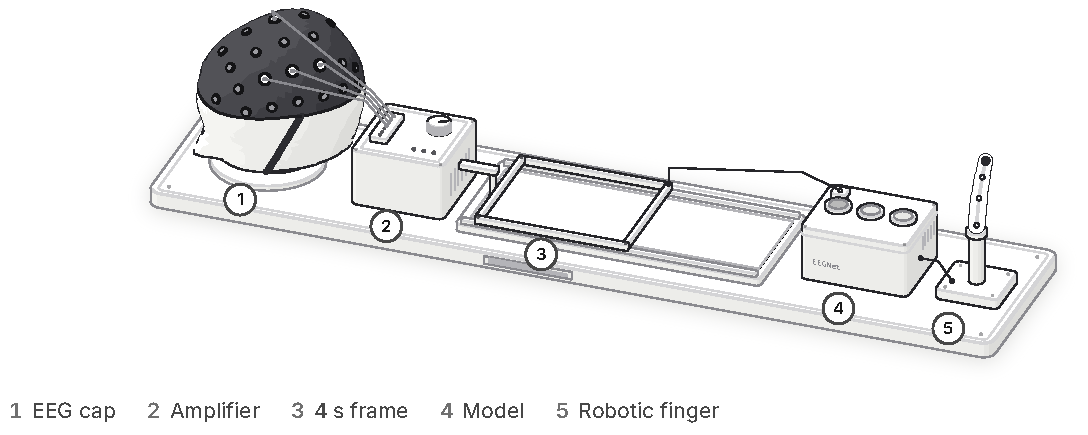
\includegraphics[width=0.8\textwidth]{web/system.pdf}
  \caption{The signal chain of a sixth-finger BCI on one bench: (1) the EEG cap, (2) the
  amplifier, (3) the 4\,s frame of signal that the decoder reads at a time, (4) the decoder,
  here EEGNet, with one lamp per class, and (5) the robotic finger it would command. In this
  study (1) and (2) are replaced by recorded EEG, and (5) is drawn on screen.}
  \label{fig:chain}
\end{figure}

\subsection{Decoding pipeline}
\label{sec:pipeline}

\emph{Input.} Each window is a matrix $X \in \mathbb{R}^{C \times T}$ with $C = 40$ channels
and $T = 1000$ samples (4\,s at \nSamplingRate\,Hz), taken from the authors' preprocessed
signals without further filtering. Windows that cross a removed segment or a run's end are discarded.

\emph{CSP with LDA.} CSP looks for spatial filters $w \in \mathbb{R}^{C}$ that extremise the
ratio of the class-conditional variances,
\begin{equation}
w^{\star} = \arg\max_{w} \frac{w^{\top} \Sigma_1 w}{w^{\top} (\Sigma_1 + \Sigma_2) w},
\label{eq:csp}
\end{equation}
where $\Sigma_1$ and $\Sigma_2$ are the mean covariance matrices of the two classes, here
estimated with Ledoit--Wolf shrinkage~\cite{ledoit2004}. Six filters are kept, ranked by
MNE's default criterion, and each window is described by the logarithm of the variance of its
six filtered signals~\cite{ramoser2000,blankertz2008}; three classes use MNE's multi-class
form of CSP~\cite{gramfort2013}. LDA with automatically chosen shrinkage then separates the
classes.

\emph{Tangent space with logistic regression (TS+LR).} Each window is summarised by its
covariance matrix $\Sigma_i$, estimated with the oracle approximating shrinkage estimator.
The matrices are projected onto the tangent space at their Riemannian mean
$\bar{\Sigma}$~\cite{barachant2012},
\begin{equation}
s_i = \mathrm{upper}\!\left( \log\!\left( \bar{\Sigma}^{-1/2} \Sigma_i \bar{\Sigma}^{-1/2}
\right) \right) \in \mathbb{R}^{C(C+1)/2},
\label{eq:ts}
\end{equation}
where $\mathrm{upper}$ keeps the upper triangle with the off-diagonal entries weighted by
$\sqrt{2}$; with 40 channels each window becomes a vector of 820 numbers. A logistic
regression with $L_2$ penalty ($C = 1$) is fitted to these vectors. MDM, a descriptive
reference, assigns each window to the class whose Riemannian mean lies nearest.

\emph{Re-centred transfer (RCT-TS+LR).} Before pooling patients, each patient $p$ is moved so
that the Riemannian mean $M_p$ of that patient's matrices becomes the
identity~\cite{zanini2018}:
\begin{equation}
\tilde{\Sigma}_i = M_p^{-1/2} \, \Sigma_i \, M_p^{-1/2}.
\label{eq:rct}
\end{equation}
The same tangent-space classifier is then trained on the other patients' re-centred windows
together with the target's, minimising
\begin{equation}
\mathcal{L} = \sum_{i \in \text{sources}} \ell(s_i, y_i) + \omega \sum_{j \in \text{target}}
\ell(s_j, y_j),
\label{eq:weight}
\end{equation}
where $\ell$ is the logistic loss and $\omega$ the weight of the target's windows. For the target, $M_p$ is estimated from the drawn windows, and at $k = 0$ from nothing but the
rest windows of runs 1--2 (\rqTwoRestMinutes\,min of unlabelled recording, nominal). The pre-registered rule chose
$\omega$ once, from $\{1, 5, 20\}$, on two development patients and without touching any run
3--4: learning on run 1 and scoring on run 2. All three candidates scored close to chance on
three classes (\rqTwoHparamRctTslrMeanMin--\rqTwoHparamRctTslrMeanMax\,\%), and the best of
them was the smallest, $\omega = \rqTwoHparamRctTslrWeight$. With it, none of the target's 80 or fewer windows weighs more than a single source window,
and the other patients supply thousands of those. Two descriptive variants ran beside it: the same classifier on the pooled
windows without re-centring (pooled TS+LR), and re-centred MDM.

\emph{EEGNet.} The network~\cite{lawhern2018} follows the braindecode
implementation~\cite{braindecode} with its default sizes (Table~\ref{tab:eegnet},
Fig.~\ref{fig:model}). Inputs are scaled from volts to microvolts. Training uses AdamW
(learning rate $10^{-3}$, weight decay $10^{-3}$), batches of 32 and cosine annealing for 150
epochs; the from-scratch network is trained with three seeds and their mean is reported. The
transfer version is first pre-trained, for each target, on all other patients after Euclidean
alignment~\cite{he2020}, which whitens each patient's windows by the inverse square root of
that patient's mean covariance; three source patients are held out for early stopping. Each
pre-trained model learned from \dlPretrainWindowsMin--\dlPretrainWindowsMax{} windows of
\dlPretrainSourcesMin--\dlPretrainSourcesMax{} patients and stopped after
\dlPretrainEpochsMin--\dlPretrainEpochsMax{} epochs. Every layer is then fine-tuned on the
target's drawn windows, aligned with the target's own reference. For fine-tuning, the same pre-registered rule picked among learning rates of $10^{-4}$ and
$3 \times 10^{-4}$ and among 20 and 50 epochs; as with the Riemannian weight, the best pair was the least adaptive one, a rate of
\rqTwoHparamEegnetLr{} for \rqTwoHparamEegnetEpochs{} epochs.

\begin{table}[!t]
  \centering
  \caption{EEGNet as used here: 40 channels, 4\,s at \nSamplingRate\,Hz, three classes.
  Shapes are (feature maps $\times$ channels $\times$ samples) for one window; the weights
  are the trainable numbers of each layer, which sum to \dlEegnetWeights.}
  \label{tab:eegnet}
  \footnotesize
  \begin{tabularx}{\textwidth}{@{}lLlr@{}}
    \toprule
    Layer & Operation & Output shape & Weights \\
    \midrule
    Input & one window, microvolts & $1 \times 40 \times 1000$ & -- \\
    Temporal convolution & 8 filters of 64 taps (0.256\,s), no bias & $8 \times 40 \times 1000$ & \dlEegnetWeightsConvTemporal \\
    Batch normalisation & scale and shift per map & $8 \times 40 \times 1000$ & \dlEegnetWeightsBnormTemporal \\
    Depthwise spatial convolution & 2 spatial filters per temporal filter, over all 40 channels & $16 \times 1 \times 1000$ & \dlEegnetWeightsConvSpatial \\
    Batch normalisation, ELU, pooling & average pooling by 4, dropout 0.25 & $16 \times 1 \times 250$ & \dlEegnetWeightsBnormOne \\
    Separable convolution, depthwise & 16 taps per map & $16 \times 1 \times 250$ & \dlEegnetWeightsConvSeparableDepth \\
    Separable convolution, pointwise & $1 \times 1$ mixing of the 16 maps & $16 \times 1 \times 250$ & \dlEegnetWeightsConvSeparablePoint \\
    Batch normalisation, ELU, pooling & average pooling by 8, dropout 0.25 & $16 \times 1 \times 31$ & \dlEegnetWeightsBnormTwo \\
    Classifier & dense layer on the 496 features, softmax & 3 & \dlEegnetWeightsClassifier \\
    \bottomrule
  \end{tabularx}
\end{table}

\begin{figure}[!t]
  \centering
  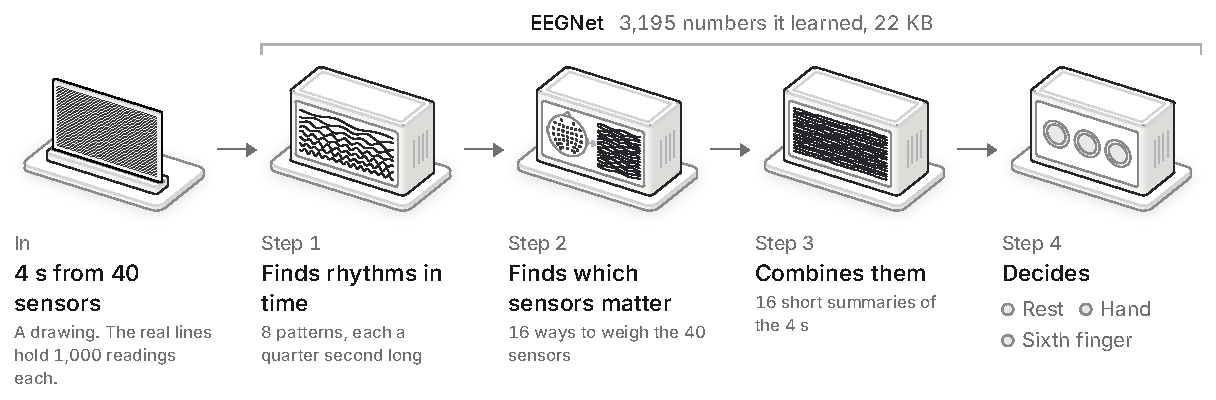
\includegraphics[width=0.86\textwidth]{web/model.pdf}
  \caption{EEGNet read as four steps: temporal filters that pick out rhythms, spatial filters
  that weigh the 40 channels, a separable stage that combines them, and the decision among
  rest, hand and sixth finger. The count printed at the top is that of the exported model
  (\demoParameters{} numbers): the export folds each batch normalisation into the
  convolution before it, so the file holds \dlEegnetWeights{} trainable weights minus one
  per normalised channel.}
  \label{fig:model}
\end{figure}

\emph{The authors' recipe, rebuilt.} To compare with the published figure we also rebuilt the
dataset's classification script: the mu-band (8--13\,Hz) power of each window in decibels
relative to the second before the cue, ten unregularised CSP filters and LDA with default
settings, with the filters fitted on all trials of the session, as the script does.

\subsection{Evaluation framework}
\label{sec:framework}

\emph{Protocols.} Trials were split in four ways. The \emph{published protocol} fits the CSP
filters on every trial of a session and then cross-validates only the classifier, ten folds
repeated ten times. \emph{Leakage-free cross-validation} uses the same folds with every step
fitted inside the training folds, so the two differ only in where the filters are fitted
(Fig.~\ref{fig:leakschema}). \emph{Leave one run out} trains on three runs and tests on the
fourth, and the \emph{chronological} split learns on runs 1--2 and tests on runs 3--4. RQ1
compares all four; every other result in this paper uses the chronological split.

\begin{figure}[!t]
  \centering
  \begin{minipage}[t]{0.485\textwidth}
  \vspace{0pt}\centering
  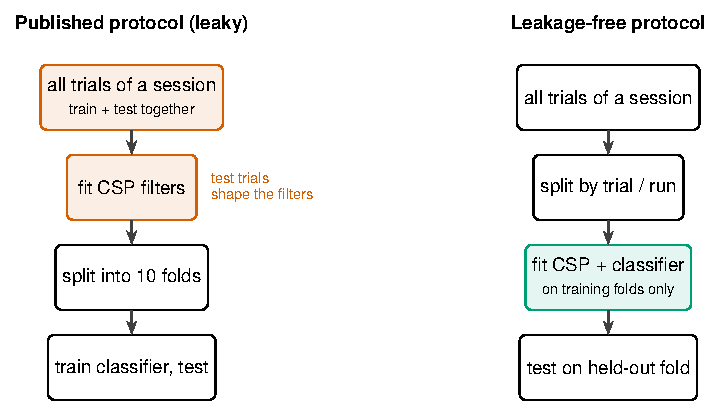
\includegraphics[width=0.86\linewidth]{fig-leakage-schematic.pdf}
  \caption{Where the leak enters. Left: in the published protocol the CSP filters are fitted
  on all trials of a session, so the test trials help to shape them before the folds are
  made. Right: in the leakage-free protocol the split comes first and the filters and the
  classifier are fitted on the training folds only. Everything else is identical.}
  \label{fig:leakschema}
  \end{minipage}\hfill
  \begin{minipage}[t]{0.485\textwidth}
  \vspace{0pt}\centering
  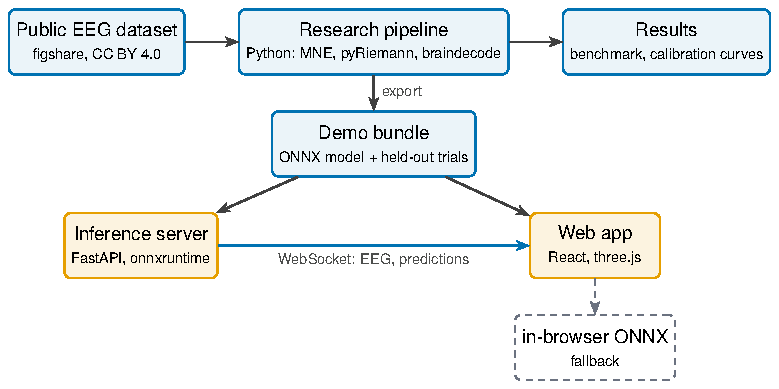
\includegraphics[width=0.95\linewidth]{fig-system-architecture.pdf}
  \caption{The demonstrator's software. A single model and the held-out trials of one
  patient leave the research pipeline as a bundle; the inference server sends them over a
  WebSocket to the web application, which can run the same ONNX model on its own whenever the
  server is unreachable.}
  \label{fig:software}
  \end{minipage}
\end{figure}

\emph{Guarding against leakage.} Before every fit the code checks that no test trial is in the
training set and that no window of the target patient, or of the target's linked partner,
is among the source data, and it stops otherwise. Unit tests exercise the check on synthetic
data. In a planned check with permuted labels, every calibration method scored near chance
on three classes (for example CSP+LDA \rqTwoNoSignalRestAhSfCspLda\,\%), as it should when
there is no signal to learn.

\emph{Hyperparameters and nesting.} The settings of every method were fixed in files before
the results. The three open transfer values ($\omega$ and the two fine-tuning values) were
chosen once by the rule above. Their source data, as in the main study, were every other
patient's windows, including those patients' runs 3--4. Those runs were therefore involved in
choosing values that were later scored on them, which slightly breaks the nesting, although the candidates ended within one point of each
other.

\emph{Provenance.} Every result row stores its commit and hashes of its settings and of the window
manifest, and every number in this paper is written by a script from the result summaries.

\subsection{Deployed system}
\label{sec:system}

The deployed system runs a trained decoder on recordings it never saw, in four parts
(Fig.~\ref{fig:software}): the research pipeline above; an export step that converts one
decoder to ONNX, an open model format, and packs it with one patient's held-out trials into a
\emph{demo bundle}; a streaming server; and a web application that draws the EEG, the
decision and a three-dimensional hand wearing the sixth finger.



\emph{The bundle.} It holds a manifest with checksums, the ONNX model, the trials as 16-bit
integers (largest error \demoQuantisationUv\,\textmu V) and the model's offline outputs; the
server refuses to start on a checksum mismatch. The demonstrator's bundle holds the \demoTrials{} complete held-out trials of \demoSubject, the patient picked by a rule set
in the protocol, and an EEGNet trained from scratch on runs 1--2 (\demoModelKb\,KB, \demoBundleMb\,MB
in all), which agrees with the trained network to within \demoParityReal{} on real windows.

\emph{The streaming server.} A FastAPI application streams each trial's phases, chunks of EEG
every 80\,ms and a prediction with its class probabilities and command whenever a window
completes: per trial on exactly the two windows the decoder was trained on, or continuously
every 0.5\,s on the last 4\,s, without knowledge of the cues, as a live device would. With ONNX Runtime on one thread of an \demoInferenceMachine{}
CPU, a decision took a median of \demoInferenceMedianMs\,ms over \demoInferenceN{} windows.

\emph{The model in the browser.} The web application picks its source of decisions itself: the server if it answers within 2\,s; otherwise the same ONNX model
run in the browser with the WebAssembly build of ONNX Runtime Web, streamed with the server's
messages and timing; otherwise the stored outputs. A badge names the active source, the
browser's outputs equal the stored ones to within $10^{-4}$, and the public site decodes in
the visitor's browser from the start.



\emph{The move-or-rest gate.} Window-by-window outputs flicker, so a command gate turns them
into stable commands. Because the results support movement against rest but not hand against
sixth finger (Sections~\ref{sec:exp} and~\ref{sec:ablation}), the page reads the decoder as a
switch: it adds the probabilities of the two movements, $q_t = P_t(\text{hand}) +
P_t(\text{sixth finger})$. The gate smooths this value,
\begin{equation}
\bar{q}_t = \alpha\, q_t + (1 - \alpha)\, \bar{q}_{t-1}, \qquad \alpha = 0.3,
\label{eq:gate}
\end{equation}
turns the finger on when $\bar{q}_t \geq 0.6$ on two consecutive decisions, and turns it off
when $\bar{q}_t$ falls below 0.45; rest is the default state. The three-class version of the pre-registered replay applies the rule to the movement class
with the highest smoothed probability; server and page share one test suite for the gate.

\emph{What is built and what is not.} The demonstrator stands in for the last two links of a
brain-controlled finger (Fig.~\ref{fig:path}). The intention, the EEG (replayed at its original speed), the processing, the decoder and the
command are the parts a physical system would also use; a live cap and amplifier, a bridge to
the decoder, and the finger's board and motor are not built. A physical system would also need filters
that use past samples only, joint and speed limits, an emergency stop with rest as the
default whenever messages stop, and per-user calibration, which is the subject of this study.
The demonstrator is not a medical device, and every screen says that the EEG is a recording.

\begin{figure}[!t]
  \centering
  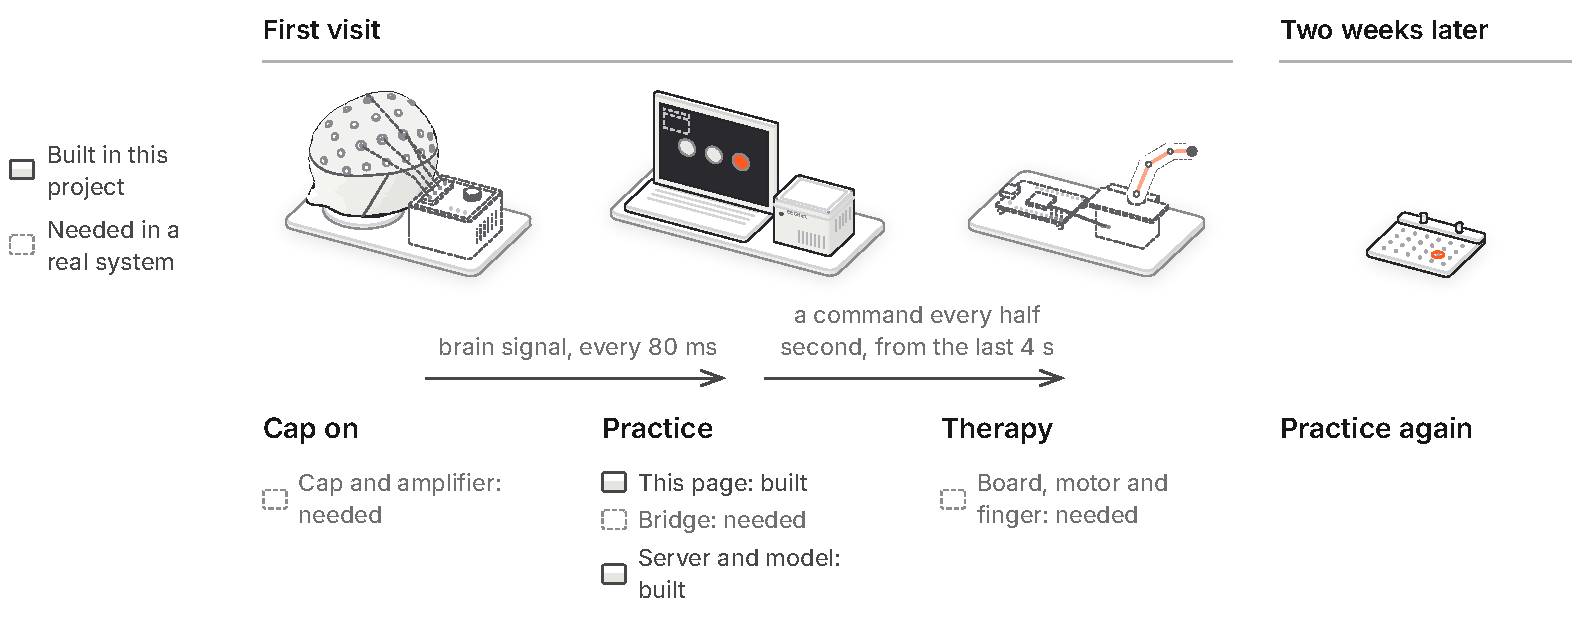
\includegraphics[width=0.86\textwidth]{web/path.pdf}
  \caption{A patient's path through a sixth-finger system, and which parts this project
  built. Solid outlines are built (the page with its model, and the model server); dashed
  outlines are still needed (the cap and amplifier, the bridge program, and the finger's
  board and motor). Along the arrows travel a chunk of EEG every 80\,ms and, every half second, a command
  decided on the latest 4\,s. Practice is repeated a fortnight later, since the decoder does
  not carry over between sessions (Section~\ref{sec:later}).}
  \label{fig:path}
\end{figure}
